\documentclass[border=10pt]{standalone}
\usepackage{tikz}\usepackage{amsmath}\usetikzlibrary{calc,arrows.meta}
\begin{document}
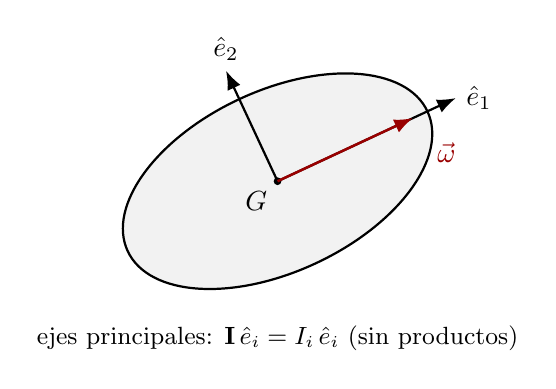
\begin{tikzpicture}[line width=0.9pt,>={Latex[length=2.4mm]}]
  % elipse de inercia
  \draw[thick,rotate=25,fill=black!5] (0,0) ellipse (2.1 and 1.15);
  % ejes principales
  \draw[->,thick] (0,0)--(25:2.5) node[right]{$\hat e_1$};
  \draw[->,thick] (0,0)--(115:1.55) node[above]{$\hat e_2$};
  \fill (0,0) circle(1.4pt) node[below left]{$G$};
  % omega y H paralelos sobre eje principal
  \draw[->,red!60!black] (0,0)--(25:1.9) node[below right=5pt]{$\vec\omega$};
  \node at (0,-2.0){\small ejes principales: $\mathbf I\,\hat e_i=I_i\,\hat e_i$ (sin productos)};
\end{tikzpicture}
\end{document}
